% Options for packages loaded elsewhere
\PassOptionsToPackage{unicode}{hyperref}
\PassOptionsToPackage{hyphens}{url}
\PassOptionsToPackage{dvipsnames,svgnames,x11names}{xcolor}
%
\documentclass[
  letterpaper,
  DIV=11,
  numbers=noendperiod]{scrartcl}

\usepackage{amsmath,amssymb}
\usepackage{lmodern}
\usepackage{iftex}
\ifPDFTeX
  \usepackage[T1]{fontenc}
  \usepackage[utf8]{inputenc}
  \usepackage{textcomp} % provide euro and other symbols
\else % if luatex or xetex
  \usepackage{unicode-math}
  \defaultfontfeatures{Scale=MatchLowercase}
  \defaultfontfeatures[\rmfamily]{Ligatures=TeX,Scale=1}
\fi
% Use upquote if available, for straight quotes in verbatim environments
\IfFileExists{upquote.sty}{\usepackage{upquote}}{}
\IfFileExists{microtype.sty}{% use microtype if available
  \usepackage[]{microtype}
  \UseMicrotypeSet[protrusion]{basicmath} % disable protrusion for tt fonts
}{}
\makeatletter
\@ifundefined{KOMAClassName}{% if non-KOMA class
  \IfFileExists{parskip.sty}{%
    \usepackage{parskip}
  }{% else
    \setlength{\parindent}{0pt}
    \setlength{\parskip}{6pt plus 2pt minus 1pt}}
}{% if KOMA class
  \KOMAoptions{parskip=half}}
\makeatother
\usepackage{xcolor}
\setlength{\emergencystretch}{3em} % prevent overfull lines
\setcounter{secnumdepth}{-\maxdimen} % remove section numbering
% Make \paragraph and \subparagraph free-standing
\ifx\paragraph\undefined\else
  \let\oldparagraph\paragraph
  \renewcommand{\paragraph}[1]{\oldparagraph{#1}\mbox{}}
\fi
\ifx\subparagraph\undefined\else
  \let\oldsubparagraph\subparagraph
  \renewcommand{\subparagraph}[1]{\oldsubparagraph{#1}\mbox{}}
\fi


\providecommand{\tightlist}{%
  \setlength{\itemsep}{0pt}\setlength{\parskip}{0pt}}\usepackage{longtable,booktabs,array}
\usepackage{calc} % for calculating minipage widths
% Correct order of tables after \paragraph or \subparagraph
\usepackage{etoolbox}
\makeatletter
\patchcmd\longtable{\par}{\if@noskipsec\mbox{}\fi\par}{}{}
\makeatother
% Allow footnotes in longtable head/foot
\IfFileExists{footnotehyper.sty}{\usepackage{footnotehyper}}{\usepackage{footnote}}
\makesavenoteenv{longtable}
\usepackage{graphicx}
\makeatletter
\def\maxwidth{\ifdim\Gin@nat@width>\linewidth\linewidth\else\Gin@nat@width\fi}
\def\maxheight{\ifdim\Gin@nat@height>\textheight\textheight\else\Gin@nat@height\fi}
\makeatother
% Scale images if necessary, so that they will not overflow the page
% margins by default, and it is still possible to overwrite the defaults
% using explicit options in \includegraphics[width, height, ...]{}
\setkeys{Gin}{width=\maxwidth,height=\maxheight,keepaspectratio}
% Set default figure placement to htbp
\makeatletter
\def\fps@figure{htbp}
\makeatother
\newlength{\cslhangindent}
\setlength{\cslhangindent}{1.5em}
\newlength{\csllabelwidth}
\setlength{\csllabelwidth}{3em}
\newlength{\cslentryspacingunit} % times entry-spacing
\setlength{\cslentryspacingunit}{\parskip}
\newenvironment{CSLReferences}[2] % #1 hanging-ident, #2 entry spacing
 {% don't indent paragraphs
  \setlength{\parindent}{0pt}
  % turn on hanging indent if param 1 is 1
  \ifodd #1
  \let\oldpar\par
  \def\par{\hangindent=\cslhangindent\oldpar}
  \fi
  % set entry spacing
  \setlength{\parskip}{#2\cslentryspacingunit}
 }%
 {}
\usepackage{calc}
\newcommand{\CSLBlock}[1]{#1\hfill\break}
\newcommand{\CSLLeftMargin}[1]{\parbox[t]{\csllabelwidth}{#1}}
\newcommand{\CSLRightInline}[1]{\parbox[t]{\linewidth - \csllabelwidth}{#1}\break}
\newcommand{\CSLIndent}[1]{\hspace{\cslhangindent}#1}

\usepackage[dvipsnames]{xcolor} % colors
\newcommand{\ear}[1]{{\textcolor{blue}{#1}}}
\newcommand{\svp}[1]{{\textcolor{RedOrange}{#1}}}
\newcommand{\rh}[1]{{\textcolor{Green}{#1}}}
% \usepackage[capitalise]{cleveref}
% \newcommand\pcref[1]{(\cref{#1})}

\usepackage{natbib}
\bibliographystyle{unsrtnat}
\KOMAoption{captions}{tableheading}
\makeatletter
\makeatother
\makeatletter
\makeatother
\makeatletter
\@ifpackageloaded{caption}{}{\usepackage{caption}}
\AtBeginDocument{%
\ifdefined\contentsname
  \renewcommand*\contentsname{Table of contents}
\else
  \newcommand\contentsname{Table of contents}
\fi
\ifdefined\listfigurename
  \renewcommand*\listfigurename{List of Figures}
\else
  \newcommand\listfigurename{List of Figures}
\fi
\ifdefined\listtablename
  \renewcommand*\listtablename{List of Tables}
\else
  \newcommand\listtablename{List of Tables}
\fi
\ifdefined\figurename
  \renewcommand*\figurename{Figure}
\else
  \newcommand\figurename{Figure}
\fi
\ifdefined\tablename
  \renewcommand*\tablename{Table}
\else
  \newcommand\tablename{Table}
\fi
}
\@ifpackageloaded{float}{}{\usepackage{float}}
\floatstyle{ruled}
\@ifundefined{c@chapter}{\newfloat{codelisting}{h}{lop}}{\newfloat{codelisting}{h}{lop}[chapter]}
\floatname{codelisting}{Listing}
\newcommand*\listoflistings{\listof{codelisting}{List of Listings}}
\makeatother
\makeatletter
\@ifpackageloaded{caption}{}{\usepackage{caption}}
\@ifpackageloaded{subcaption}{}{\usepackage{subcaption}}
\makeatother
\makeatletter
\@ifpackageloaded{tcolorbox}{}{\usepackage[many]{tcolorbox}}
\makeatother
\makeatletter
\@ifundefined{shadecolor}{\definecolor{shadecolor}{rgb}{.97, .97, .97}}
\makeatother
\makeatletter
\makeatother
\ifLuaTeX
  \usepackage{selnolig}  % disable illegal ligatures
\fi
\IfFileExists{bookmark.sty}{\usepackage{bookmark}}{\usepackage{hyperref}}
\IfFileExists{xurl.sty}{\usepackage{xurl}}{} % add URL line breaks if available
\urlstyle{same} % disable monospaced font for URLs
\hypersetup{
  pdftitle={`You Draw It': Implementation of visually fitted trends with r2d3},
  pdfkeywords={graphics, user interaction, regression},
  colorlinks=true,
  linkcolor={blue},
  filecolor={Maroon},
  citecolor={Blue},
  urlcolor={Blue},
  pdfcreator={LaTeX via pandoc}}

\title{`You Draw It': Implementation of visually fitted trends with
\texttt{r2d3}}
\author{}
\date{}

\begin{document}
\maketitle
\begin{abstract}
How do statistical regression results compare to intuitive, visually
fitted results? Fitting lines by eye through a set of points has been
explored since the 20th century. Common methods of fitting trends by eye
involve maneuvering a string, black thread, or ruler until the fit is
suitable, then drawing the line through the set of points. In 2015, the
New York Times introduced an interactive feature, called `You Draw It,'
where readers are asked to input their own assumptions about various
metrics and compare how these assumptions relate to reality. This
research is intended to implement `You Draw It', adapted from the New
York Times, as a way to measure the patterns we see in data.
\end{abstract}
\ifdefined\Shaded\renewenvironment{Shaded}{\begin{tcolorbox}[interior hidden, boxrule=0pt, frame hidden, borderline west={3pt}{0pt}{shadecolor}, enhanced, sharp corners, breakable]}{\end{tcolorbox}}\fi

\hypertarget{introduction}{%
\section{Introduction}\label{introduction}}

We all use statistical graphics, but how do we know that the graphics we
use are communicating effectively? Through experimentation, graphical
testing methods allow researchers to conduct studies designed to
understand how we perceive graphics and perform graphical tasks such as
differentiation, prediction, estimation, and extrapolation. Each of
these levels of interaction with a graph require a different method of
engagement with and use of the information presented in a chart. In this
paper, we describe the adaptation of an old tool for graphical testing
and evaluation, eye-fitting, for use in modern web-applications suitable
for testing statistical graphics. We present an empirical evaluation of
this testing method for linear regression, and briefly discuss an
extension of this method to non-linear applications.

One of the most common charts created is a scatter plot of points over
time; these charts show up regularly in news articles and in scientific
publications alike. These charts rely on our ability to identify and
detect trends in data. Our visual system is naturally built to look for
structure and identify patterns, including patterns and trends over
time; many times we do not even notice this process happening
subconsciously. As shown in Figure~\ref{fig-gas-prices}, a viewer
engaging with a plot of weekly average gas prices over time may perform
several cognitive operations. First, they scan the plot and assesses
points to determine if there are any outliers or otherwise remarkable
points. Then, they may fit a rough mental smooth/trend line to the
points to summarize the useful information and remove variability.
Finally, an interested and engaged viewer may pull in additional
contextual information from long-term memory, seeking to explain
variation in the mental `trend' with supplemental information, such as
COVID lock downs which reduced gasoline demand and the beginning of the
war in Ukraine, which wreaked havoc on the supply and demand for global
energy sources.

\begin{figure}

{\centering 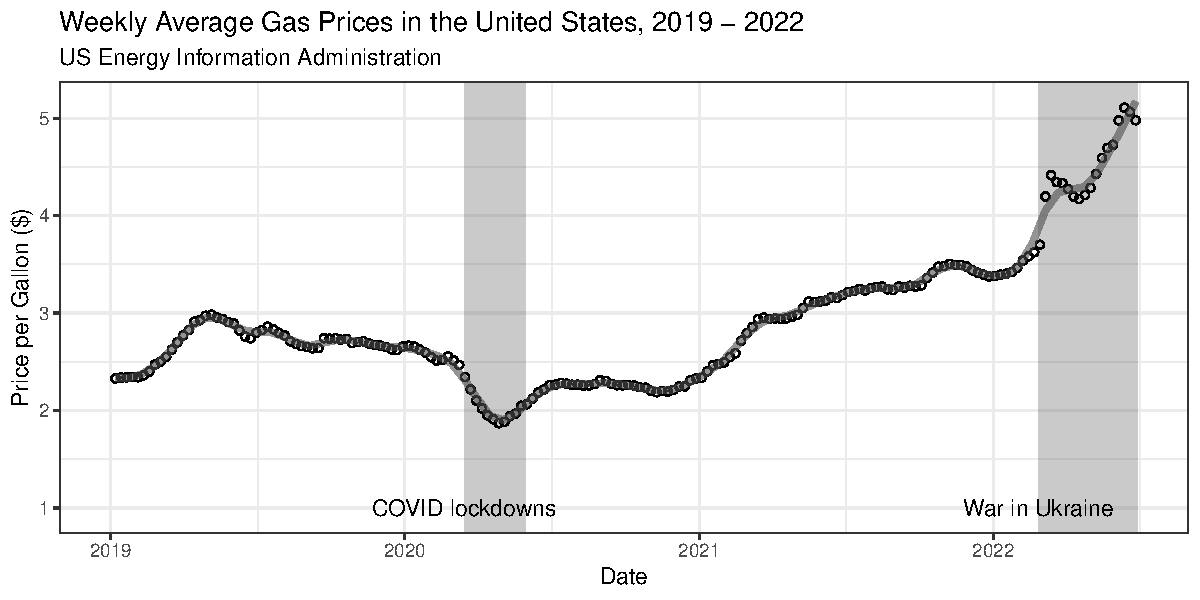
\includegraphics{./images/fig-gas-prices-1.pdf}

}

\caption{\label{fig-gas-prices}Weekly average gas prices in the United
States, 2019-June 2022. Additional mental operations a viewer might
perform while looking at the plot are annotated in grey. US Energy
Information Administration (2022)}

\end{figure}

Initial studies in the 20th century explored the use of fitting lines by
eye through a set of points Mosteller et al. (1981). Common methods of
fitting trends by eye involved maneuvering a string, black thread, or
ruler until the fit was suitable, then drawing the line through the set
of points.
\ear{Results from these early studies provided groundwork for visually judging slopes and selecting accurate starting values for common iterative calculations.}
Recently, Ciccione and Dehaene (2021) conducted a comprehensive set of
studies investigating human ability to detect trends in graphical
representations from a psychophysical approach.
\ear{This set of studies asked participants to judge trends, estimate slopes, and conduct extrapolation by using a track-pad to adjust the tilt of a line on the screen. 
Results indicated the slopes participants reported were always in excess of the ideal slopes, both in the positive and in the negative direction, and those biases increased with noise and with number of points. 
This supported the results found in @mosteller1981eye and suggested that participants might use Deming regression [@deming1943statistical], which minimizes the Euclidean distance of points from the line, when fitting a line to a noisy scatter-plot.}

While psychologists and statisticians have been using eye-fitting
techniques to assess our innate perceptual statistical modeling
abilities, news organizations have used similar techniques in order to
draw readers in and demonstrate the difference between readers'
assumptions and reality. In 2015, the New York Times introduced an
interactive feature, called `You Draw It' (Aisch, Cox, and Quealy 2015),
where readers input their own assumptions about various metrics of news
interest and compare these assumptions to reality. The New York Times
team used Data Driven Documents (D3), a JavaScript library that allows
readers to interact with a chart directly by drawing a line on their
computer screen with a mouse. Despite the somewhat different purpose
behind this feature, the D3 driven method used by the NYT is wonderfully
intuitive, and does not require the assumption of linearity, making it
much more adaptable to testing how viewers perceive and predict when
presented with non-linear data.

We set out to implement `You Draw It', adapted from the New York Times
feature, as a way to experimentally assess the patterns we see in data.
Here, we provide technical details of the software development,
utilizing interactive graphics in R (R Core Team 2022). We then share
results from our study which validates `You Draw It' as a method for
graphical testing on linear trends and apply an appropriate data
analysis method to the participant data. We also briefly demonstrate the
use of the `You Draw It' method and analysis on nonlinear data.

\hypertarget{development}{%
\section{Development}\label{development}}

\hypertarget{you-draw-it-v0}{%
\subsection{You Draw It v0}\label{you-draw-it-v0}}

\svp{Describe the NYT code - what it does, how it works (for loop to connect mouse coordinates to closest point via inverting the scales)}

The New York Times uses D3, Data Driven Documents (Bostock, Ogievetsky,
and Heer 2011), to create many of the interactive data graphics that
users rely on, from the famous ``election needle'' in 2016 to their
COVID dashboards. Naturally, this same framework was used to create the
`You Draw It' feature.

A challenge of working with D3 is the environment necessary to display
the graphics and images.
\ear{Typically, a server setup is needed in order to render D3 visuals and show output from JavaScript on the webpage.
This can be a barrier to getting started with D3 for someone unfamiliar with server setup and minimal JavaScript coding background.
Resources, such as @wattenberger-fullstack, help novice users overcome this challenge by walking them step by step through setting up a local server and creating their first plot in D3.
In the next section, we will see how the `r2d3` package [@r2d3pkg] in R can be used to display D3 visuals in familiar R HTML formats such as Rmarkdown and Shiny.}

\hypertarget{generating-d3-plots-in-r}{%
\subsection{Generating D3 Plots in R}\label{generating-d3-plots-in-r}}

\svp{Describe the process of using `r2d3`}

We leveraged the \texttt{r2d3} package to take data randomly generated
in R and create a D3 plot that could be modified with the You Draw It
script. This step allowed us to more easily connect the data generation
process with the resulting D3 code without having to generate new code
manually each time we re-generated the data. While not strictly
necessary for the validation test of the `You Draw It' method compared
to past linear regression methods presented in this paper, this
abstraction makes it much easier to test arbitrary or model-generated
data which is unique to each participant.

We conducted all data simulation and processing in R and output two data
sets - \emph{point data} and \emph{line data} - containing (x, y)
coordinates corresponding to either a simulated point or fitted value
predicted by a statistical model respectively. Then, the \texttt{r2d3}
package converts the data sets in R to JavaScript Object Notation (JSON)
to be interpreted by JavaScript code included with the \texttt{r2d3}
package. Parameters for aesthetic design choices are defined in a list
of options in the \texttt{r2d3} function call; \texttt{r2d3} passes
these to the generated JavaScript code. For instance, we can specify the
buffer space allowed for the \(x\) and \(y\) axes to avoid users
anchoring their lines to the axes limits.

\hypertarget{modifying-you-draw-it}{%
\subsection{Modifying You Draw It}\label{modifying-you-draw-it}}

In order to make use of the original `You Draw It' code for perceptual
experiments, we first needed to accommodate an additional layer. The
original NYT features asked participants to draw on a blank coordinate
grid, as shown in Figure~\ref{fig-nyt-screenshot}.

\begin{figure}

{\centering 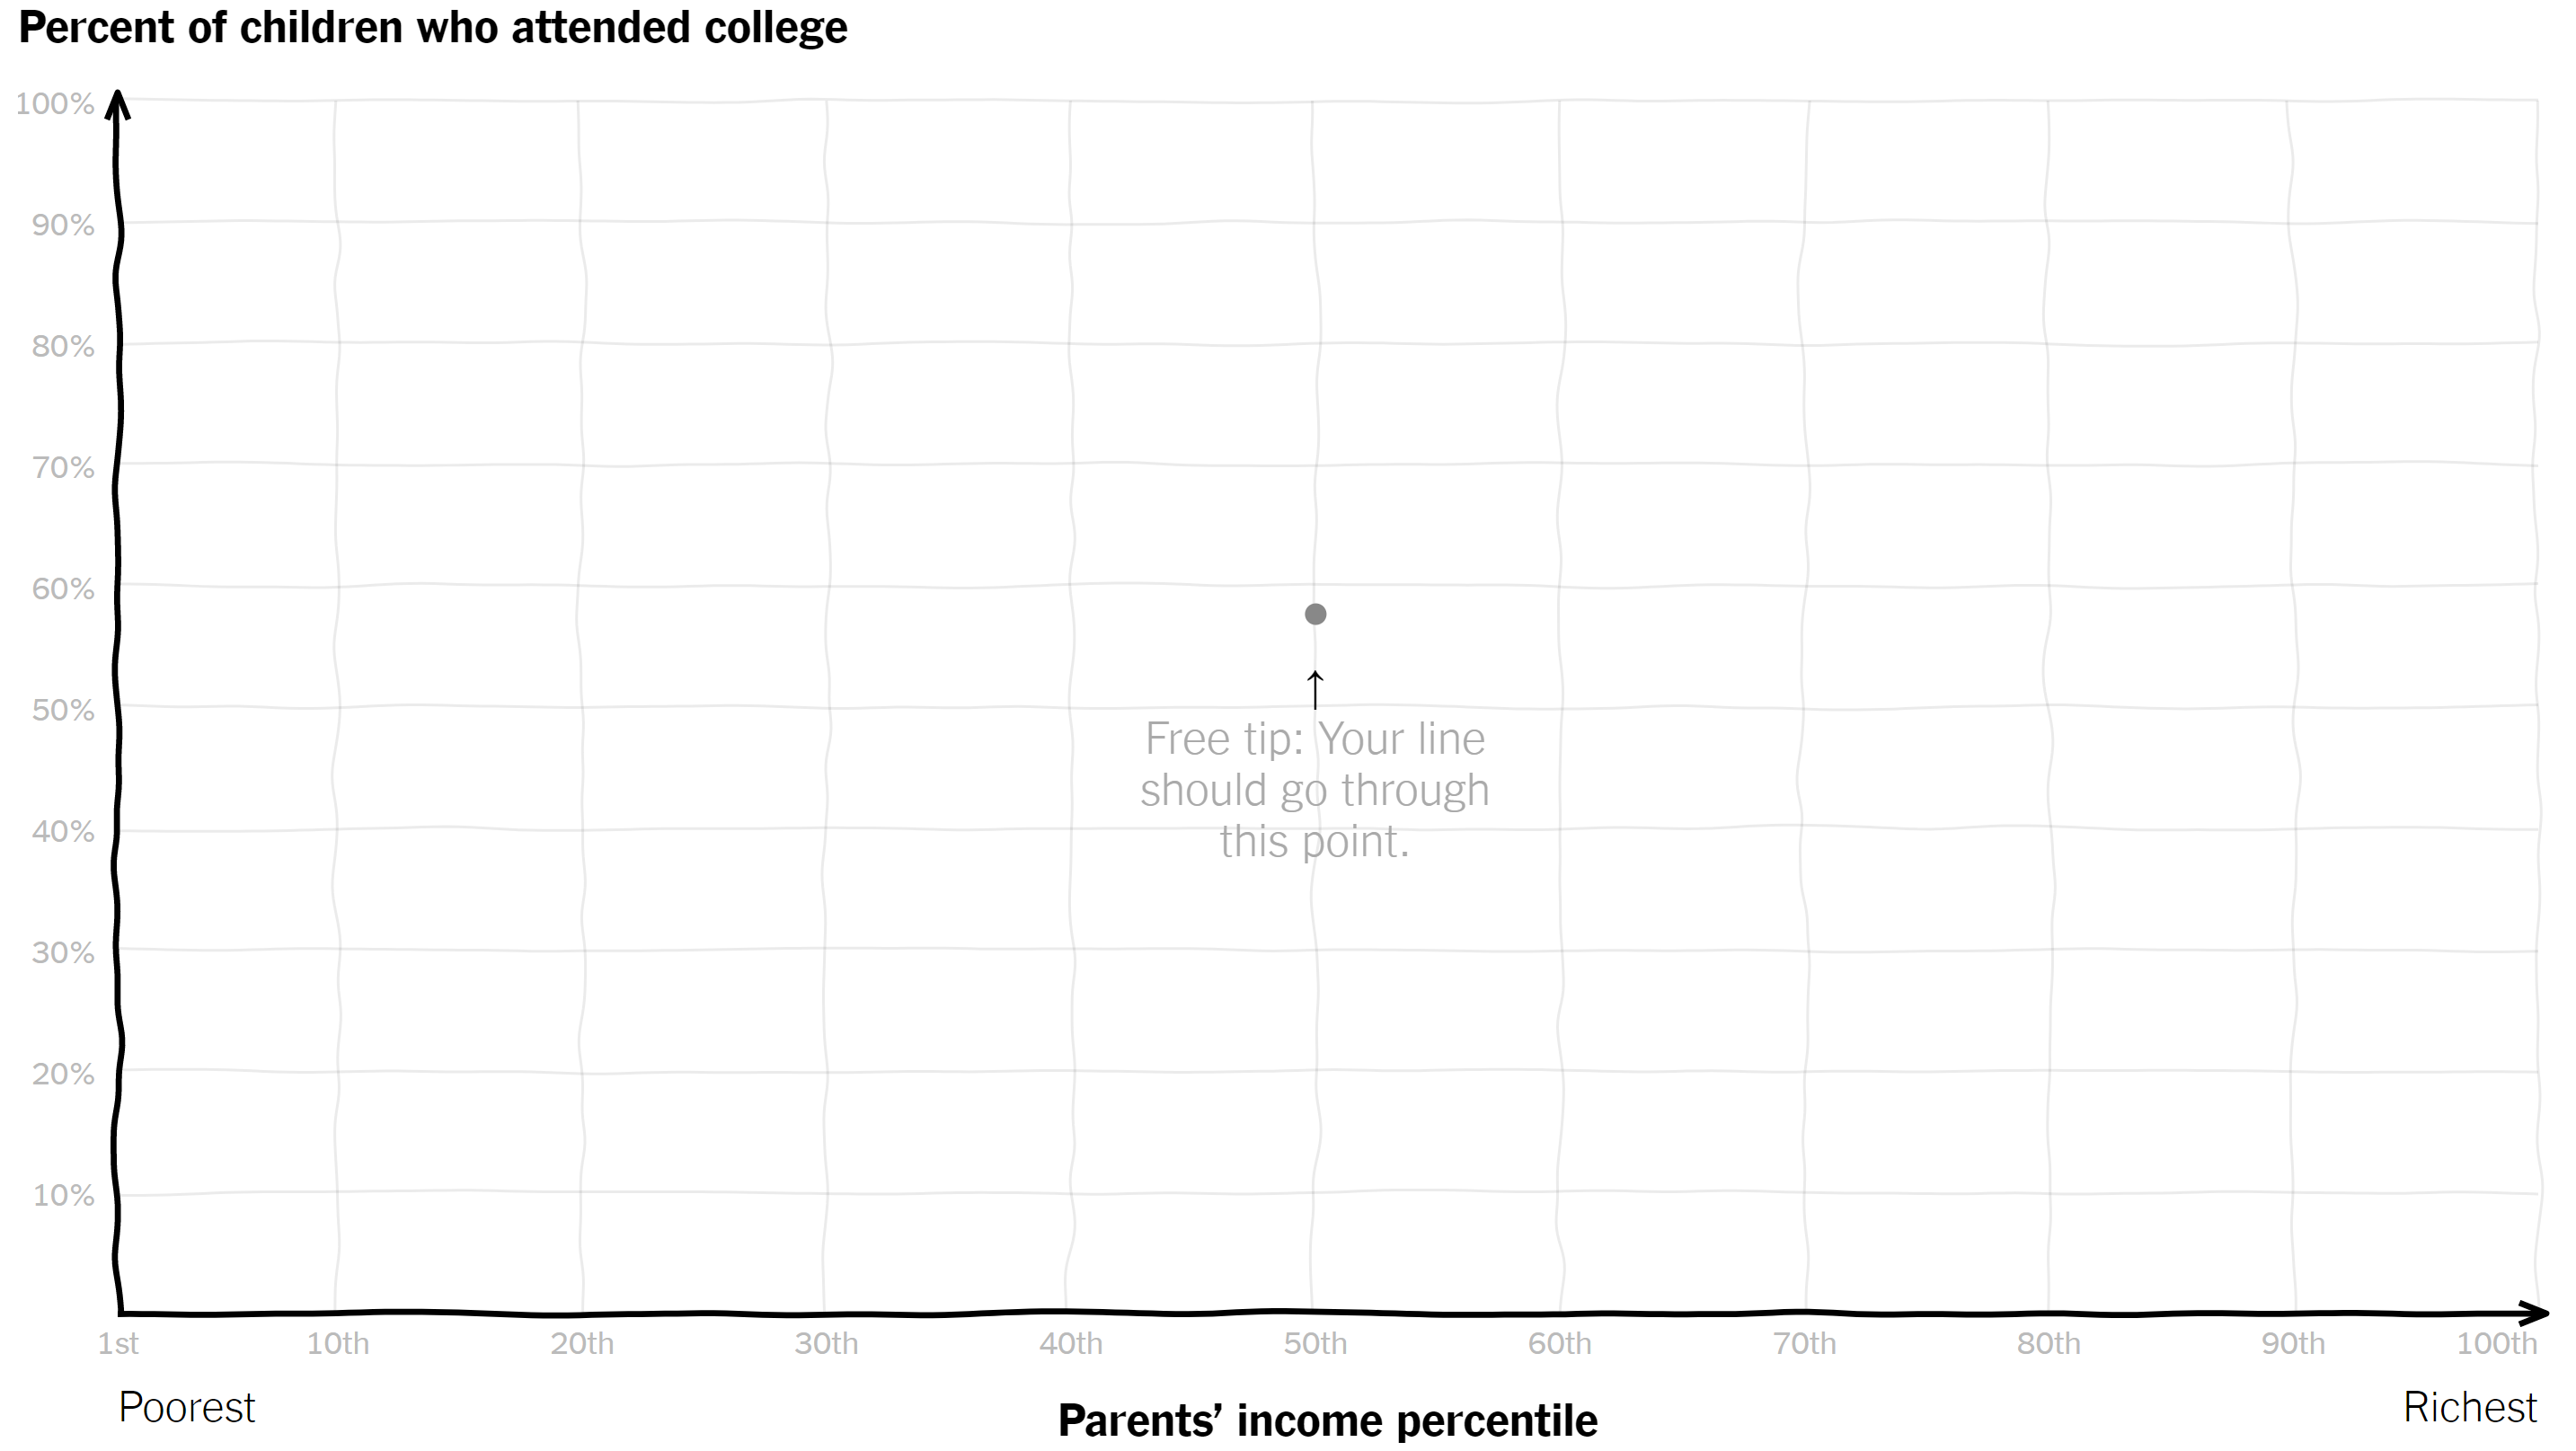
\includegraphics{images/NYT-You-Draw-It-Screenshot.png}

}

\caption{\label{fig-nyt-screenshot}Screenshot of the
\href{https://www.nytimes.com/interactive/2015/05/28/upshot/you-draw-it-how-family-income-affects-childrens-college-chances.html}{You
Draw It application} originally developed by the New York Times.}

\end{figure}

When testing perception of graphics, however, we want to pre-populate
the chart with additional information - points, and in some cases,
portions of a trend line. This requires that we modify the original
JavaScript \ear{source} code to accommodate these additional elements,
which we generate using \texttt{r2d3}, as described above.

We defined JavaScript functions to draw the initial plot and set up
drawable points for the user drawn line. Drag events in \texttt{D3.js}
are utilized to observe and react to user input, as in the original `You
Draw It' script from the NYT. \footnote{The full source code we
  developed for the YouDrawIt task is available at
  \url{https://github.com/earobinson95/presentations/blob/master/can-you-draw-it/www/main-d3v5.js}.}

One constraint we inherited from the NYT code is that users can only
draw one-to-one functions; because the code works with drag events, each
point in \(x\) can correspond to only one point in \(y\), at least as
the code is currently written. While this is not particularly
problematic for our applications to date, it might limit applications of
this type of user interaction when assessing user drawn confidence
bands, ribbons, and other situations where two or more vertical points
are required.

\hypertarget{visual-cues}{%
\subsection{Visual Cues}\label{visual-cues}}

During testing of our modifications to the You Draw It' script, we
discovered that frequently the JavaScript code would ``skip'' from point
to point out of sequence. This resulted in a jagged line (visually) with
missing values in the underlying stored array of data; as a result, the
for-loop controlling the user-drawn line never exited and the user's
data was not recorded. While it would have been possible to fix this
using some sort of interpolation algorithm, we did not want to
compromise user results by introducing interpolation artifacts, so we
opted instead for a visual cue that fixed the problem from a
psychological angle.

\begin{figure}

{\centering 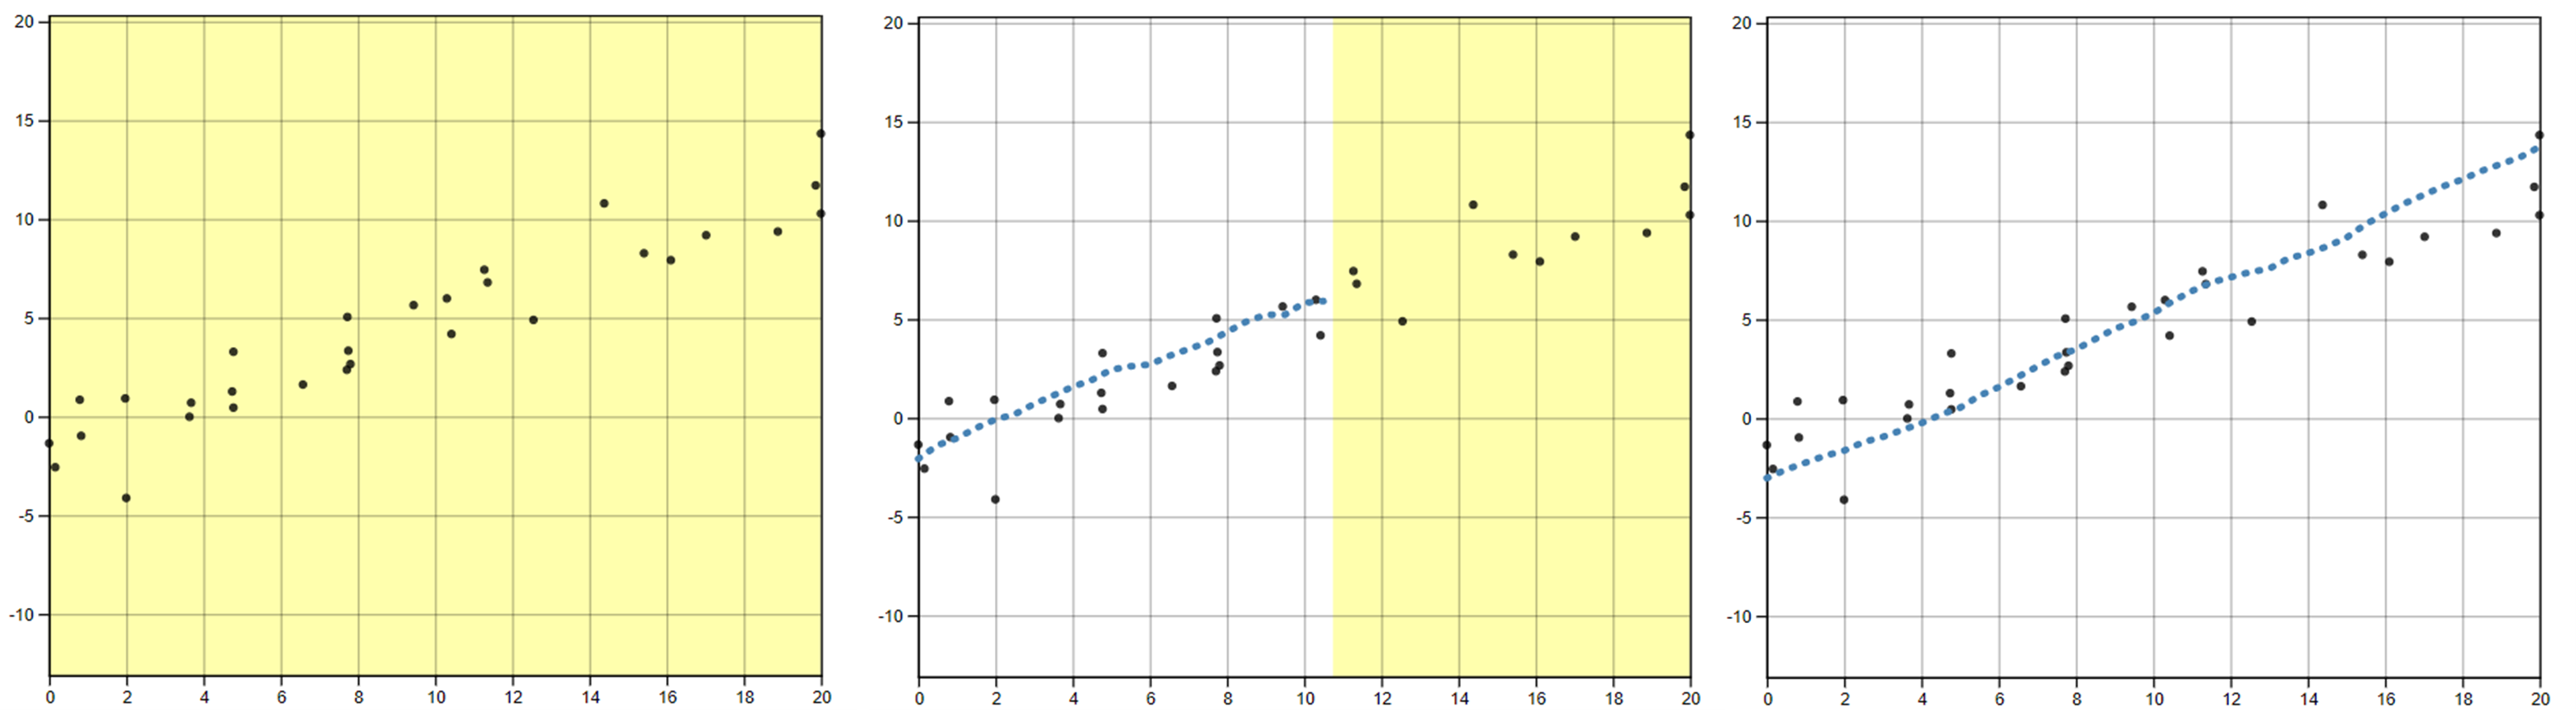
\includegraphics{images/ydi-stimuli.png}

}

\caption{\label{fig-you-draw-it-task-plot}You Draw It task plot as shown
to user.\\
\textbf{left:} Initial state, with instructions \emph{Use your mouse to
fill in the trend in the yellow box region.}\\
\textbf{middle:} User view during task completion.\\
\textbf{right:} Finished state}

\end{figure}

As shown in Figure~\ref{fig-you-draw-it-task-plot}, the user-filled
portion of the plot is represented with a yellow rectangle, which adapts
to the user's input and spans any missing values. When the box
disappears, the array is filled in and the user can submit their
response.

One challenge introduced by adding this visual cue is that D3 uses
Scalable Vector Graphics (SVG) to render elements. Adding an additional
layer meant that we had to ensure that not only the grids, lines, and
points of the default scatter plot and trend line rendered in the
correct order, but that the yellow box rendered behind all of these
points as well so that no information was masked.

\hypertarget{connecting-to-shiny}{%
\subsection{Connecting to Shiny}\label{connecting-to-shiny}}

Shiny Messages are used to communicate the user interaction between the
JavaScript code and the R environment. The initial plot is rendered
using Shiny's \texttt{RenderD3} and \texttt{d3Output} functions;
subsequent user interactions are controlled via the JavaScript code.
Once the user is finished modifying the plot, they can submit their
response, so long as they have filled in all of the points. This is
enforced using Shiny's message-passing interface and a hook in the
JavaScript code that notifies Shiny when the array of user-drawn points
is completely filled in. Once the user is done drawing the line, we save
the results of the drawn line to a SQLite database, using Shiny to pass
data from JavaScript to R. The connections between each portion of the
app are shown in Figure~\ref{fig-you-draw-it-code-sketch}.

\begin{figure}

{\centering 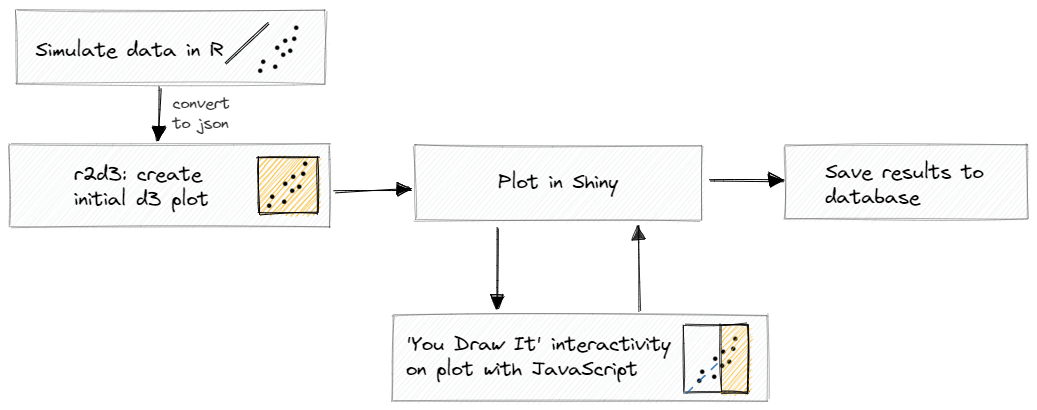
\includegraphics{images/code-sketch-2.png}

}

\caption{\label{fig-you-draw-it-code-sketch}Sketch of underlying code
for `You Draw It', illustrating the data simulation conducted in R, the
initial setup of the visual stimuli with D3 source code, along with the
iterative process between the user interaction and plotting in Shiny.
Once the user is done drawing the line, we saved the results of the
drawn line to a database for analysis.}

\end{figure}

One additional challenge when integrating the D3 graphics into the Shiny
application is that by default, most Shiny applications use a reactive
framework that adjusts to the user's browser size. When working with D3,
however, this can be problematic: most D3 parameters are specified at
the pixel level. The discontinuity between the assumptions of Shiny and
D3 meant that we had to fix the size of the Shiny element, and then
perform a check to ensure that the user's screen was sufficiently big to
render the plot. While in an ideal world, users could participate using
cell phones, tablets, and traditional laptop/desktop computers,
functionally our checks limited users' ability to participate using
smaller screen sizes found in cell phones and some tablets.
Additionally, after some feedback by laptop users during pilot testing,
we included an additional requirement that participants have a computer
mouse available; the results from touchpad users were qualitatively
different (more jagged) in ways suggesting that the recorded data did
not adequately describe users' perceptions.

\hypertarget{application}{%
\section{Application}\label{application}}

\hypertarget{validation-study}{%
\subsection{Validation Study}\label{validation-study}}

We conducted a study in order to validate `You Draw It' as a method for
graphical testing, comparing results to the less technological method
utilized in Mosteller et al. (1981). The original study asked 153
graduate students and postdoctoral researchers in an Introductory
Biostatistics course to fit lines by eye to a set of four points (S, F,
V, N), each set with differing slope and variance properties, using an
8.5 x 11 inch transparency with a straight line etched across the
middle. Researchers conducted the study with a latin square experimental
design to test for a practice effect on the task. Results indicated
participants tended to fit the slope of the first principal component
(minimizes orthogonal residuals) as opposed to the slope from the
ordinary least squares regression (minimizes vertical residuals)
Figure~\ref{fig-pca-plot} and found no effect of order.

\begin{figure}

{\centering 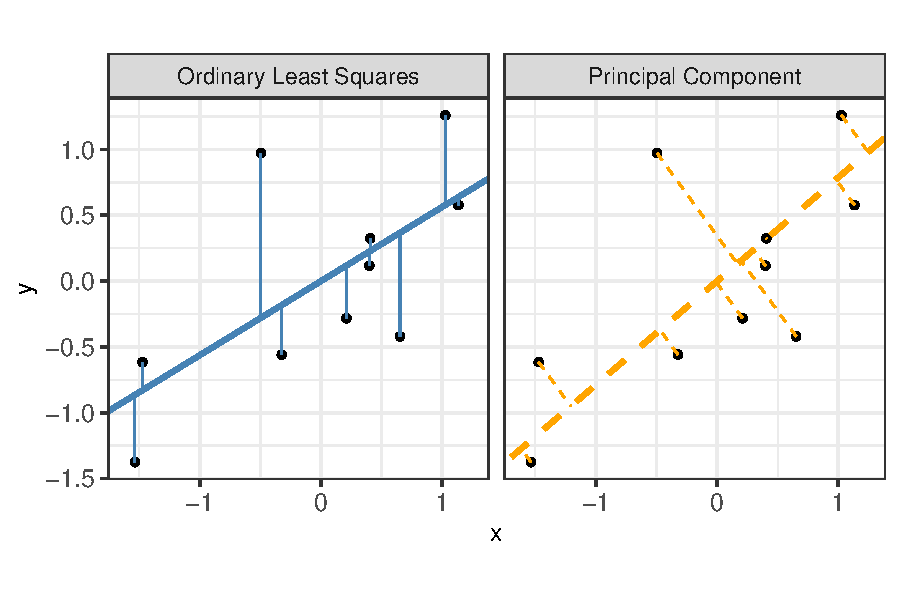
\includegraphics{./images/fig-pca-plot-1.pdf}

}

\caption{\label{fig-pca-plot}Comparison between an OLS regression
equation which minimizes the vertical distance of points from the line
and a regression equation with a slope calculated by the first principal
component which minimizes the smallest distance of points from the
line.}

\end{figure}

In our study, we replicated Mosteller et al. (1981) using the `You Draw
It' method and simulated data with parameter coefficients selected to
reflect those from the four data sets in the original study. Data were
simulated based on a linear model with additive errors: \begin{align}
y_i & = \beta_0 + \beta_1 x_i + e_i \\
\text{with } e_i & \sim N(0, \sigma^2). \nonumber
\end{align} For each participant, a unique data set was randomly and
independently generated from the underlying parameters at the beginning
of the study and mapped to a scatter-plot graphic.
Figure~\ref{fig-eyefitting-simplot} illustrates an example of simulated
data for all four parameter choices intended to reflect the trends in
the original study. When participants started the study, they were first
asked to complete two practice plots - accompanied by instructions and a
.gif demonstrating the task - in order to train them in the skills
associated with executing the task. The four `You Draw It' task plots
associated with the selected parameters followed the practice plots in a
random order for each individual.

\begin{figure}

{\centering 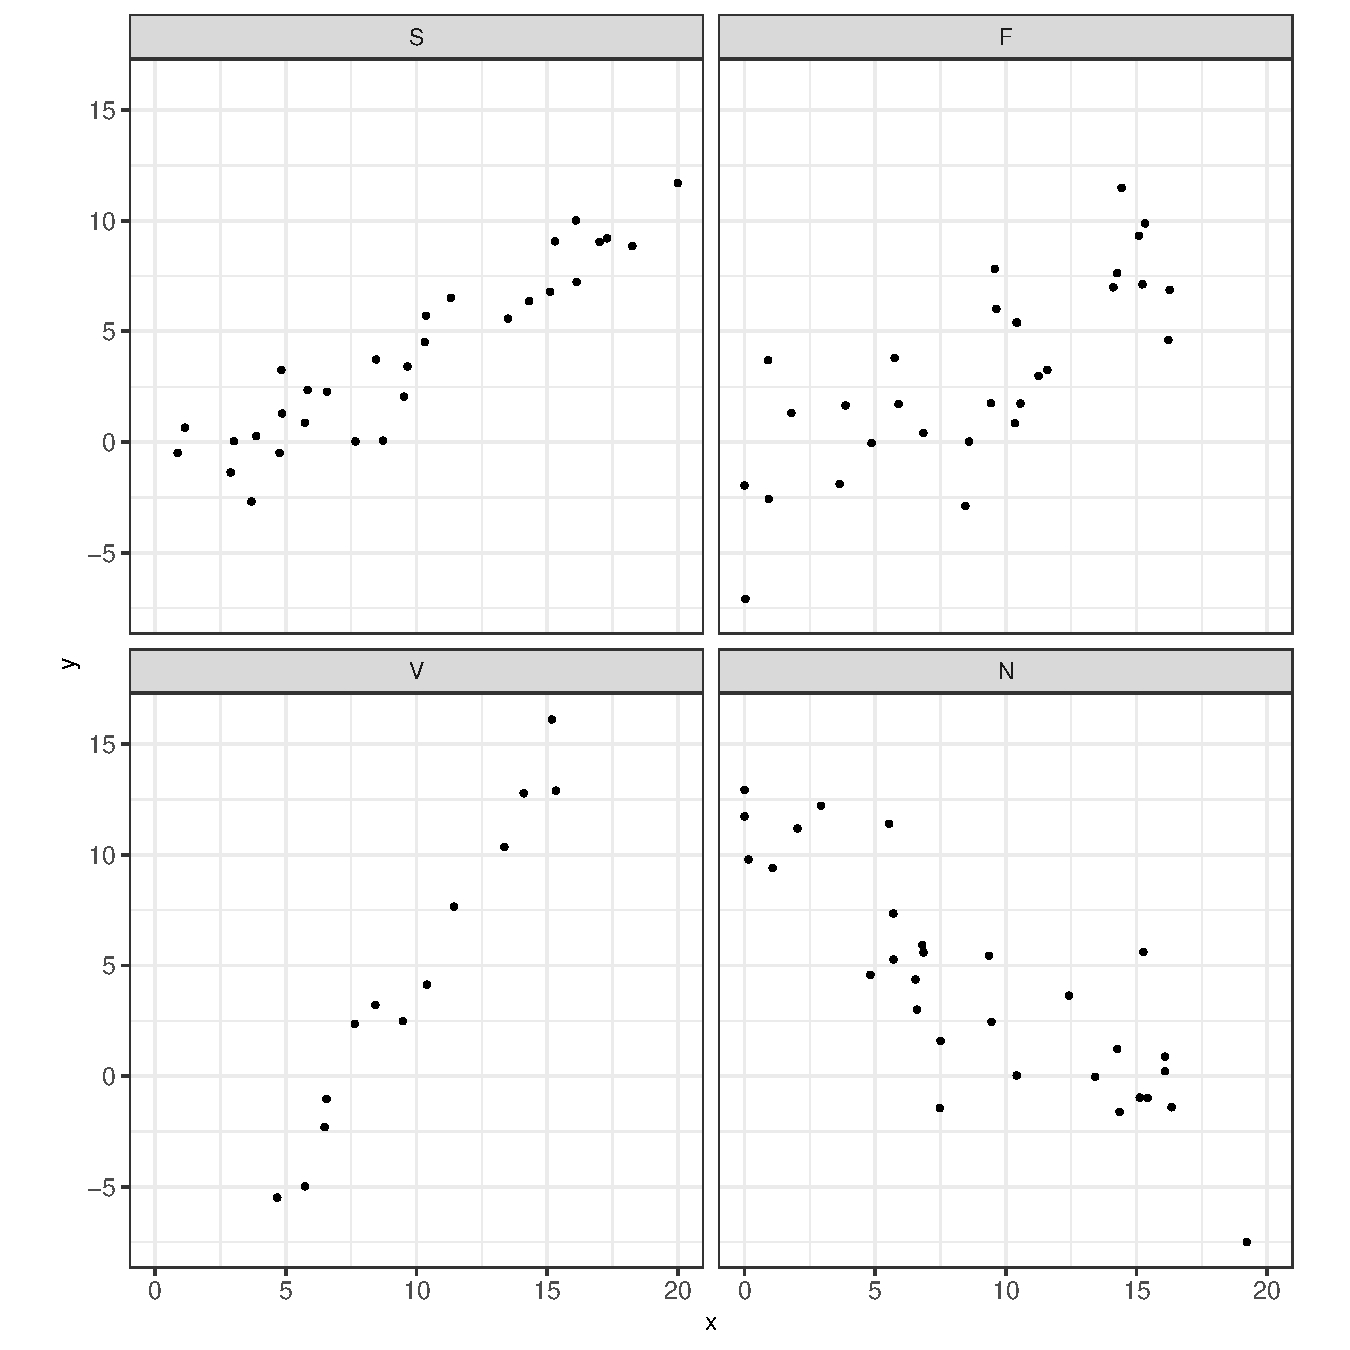
\includegraphics{./images/fig-eyefitting-simplot-1.pdf}

}

\caption{\label{fig-eyefitting-simplot}Example of simulated data points
displayed in a scatter-plot illustrating the trends associated with the
four selected parameter choices.}

\end{figure}

Participants were recruited via Prolific in March 2022; while this study
does utilize a convenience sample, as this is primarily a perceptual
task, previous results have found few differences between expert and
non-expert participants in this context {[}CITE SPATIAL PAPER{]}. The
study was conducted and distributed via a Shiny application and
participants completed the tasks on their own computer, with a computer
mouse, and in an environment of their choosing. The data from this study
were collected to validate this method of graphical testing, with the
hopes of providing a new tool to assess graphical perception
interactively.

\hypertarget{data-analysis-and-results}{%
\subsection{Data Analysis and Results}\label{data-analysis-and-results}}

As a part of the validation study, we collected data for each
participant drawn trend line, allowing us to conduct formal analyses
which compared the intuitive visually fit lines to statistical
regression results - the original study lacked these formal comparisons,
providing only summaries of averages, variances, and actual (least
squares) values for the slope and intercept of each data set. The
feedback data, stored in a SQLite database, contained the simulated data
points\} - \((x_{ijk}, y_{ijk})\) -, the predicted values from the
statistical regression models - \(\hat y_{ijk,OLS}\), and
\(\hat y_{ijk,PCA}\) -, and the predicted values from the user drawn
line - \(y_{ijk,drawn}\) for parameter choice \(i = 1,2,3,4\),
\(j = 1,...N_\text{participant}\), and \(x_{ijk}\) value
\(k = 1, ...,4 x_{max} + 1\). Figure~\ref{fig-eyefitting-trial-plot}
displays an example of all three fitted trend lines for parameter choice
F.

\begin{figure}

{\centering 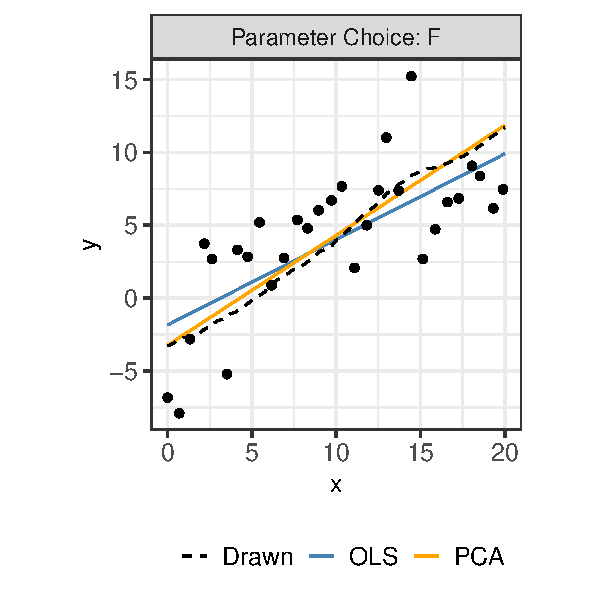
\includegraphics{./images/fig-eyefitting-trial-plot-1.pdf}

}

\caption{\label{fig-eyefitting-trial-plot}Example of validation feedback
data where three trend lines show the the OLS fitted, PCA fitted, and
participant drawn values overlaid on the simulated data points.}

\end{figure}

A unique data set was simulated independently for each participant,
therefore, comparisons of vertical residuals between the user drawn line
and the OLS fitted values
(\(e_{ijk,OLS} = y_{ijk,drawn} - \hat y_{ijk,OLS}\)) and PCA fitted
values (\(e_{ijk,PCA} = y_{ijk,drawn} - \hat y_{ijk,PCA}\)) were used to
assess the accuracy of participant drawn lines. We use mixed model
methods to analyze residual trends and capture the variability due to
participant differences.

We first fit a linear mixed model (LMM) to the OLS and PCA residuals
separately using the \texttt{lmer} function in the \texttt{lme4} package
(Bates et al. 2015), constraining the fit to a linear trend. Parameter
choice, \(x\), and the interaction between \(x\) and parameter choice
were treated as fixed effects with a random participant effect
accounting for variation due to participant. The LMM equation for each
fit (OLS and PCA) residuals is given by: \begin{equation}
y_{ijk,drawn} - \hat y_{ijk,fit} = e_{ijk,fit} = \left[\gamma_0 + \alpha_i\right] + \left[\gamma_{1} x_{ijk} + \gamma_{2i} x_{ijk}\right] + p_{j} + \epsilon_{ijk}
\end{equation} \noindent where

\begin{itemize}
\tightlist
\item
  \(y_{ijk,drawn}\) is the drawn y-value for the \(i^{th}\) parameter
  choice, \(j^{th}\) participant, and \(k^{th}\) increment of
  \(x\)-value
\item
  \(\hat y_{ijk,fit}\) is the fitted y-value for the \(i^{th}\)
  parameter choice, \(j^{th}\) participant, and \(k^{th}\) increment of
  \(x\)-value corresponding to either the OLS or PCA fit
\item
  \(e_{ijk,fit}\) is the residual between the drawn and fitted y-values
  for the \(i^{th}\) parameter choice, \(j^{th}\) participant, and
  \(k^{th}\) increment of \(x\)-value corresponding to either the OLS or
  PCA fit
\item
  \(\gamma_0\) is the overall intercept
\item
  \(\alpha_i\) is the effect of the \(i^{th}\) parameter choice (F, S,
  V, N) on the intercept
\item
  \(\gamma_1\) is the overall slope for \(x\)
\item
  \(\gamma_{2i}\) is the effect of the parameter choice on the slope
\item
  \(x_{ijk}\) is the \(x\)-value for the \(i^{th}\) parameter choice,
  \(j^{th}\) participant, and \(k^{th}\) increment
\item
  \(p_{j} \sim N(0, \sigma^2_\text{participant})\) is the random error
  due to the \(j^{th}\) participant's characteristics
\item
  \(\epsilon_{ijk} \sim N(0, \sigma^2)\) is the residual error.
\end{itemize}

\begin{figure}

{\centering 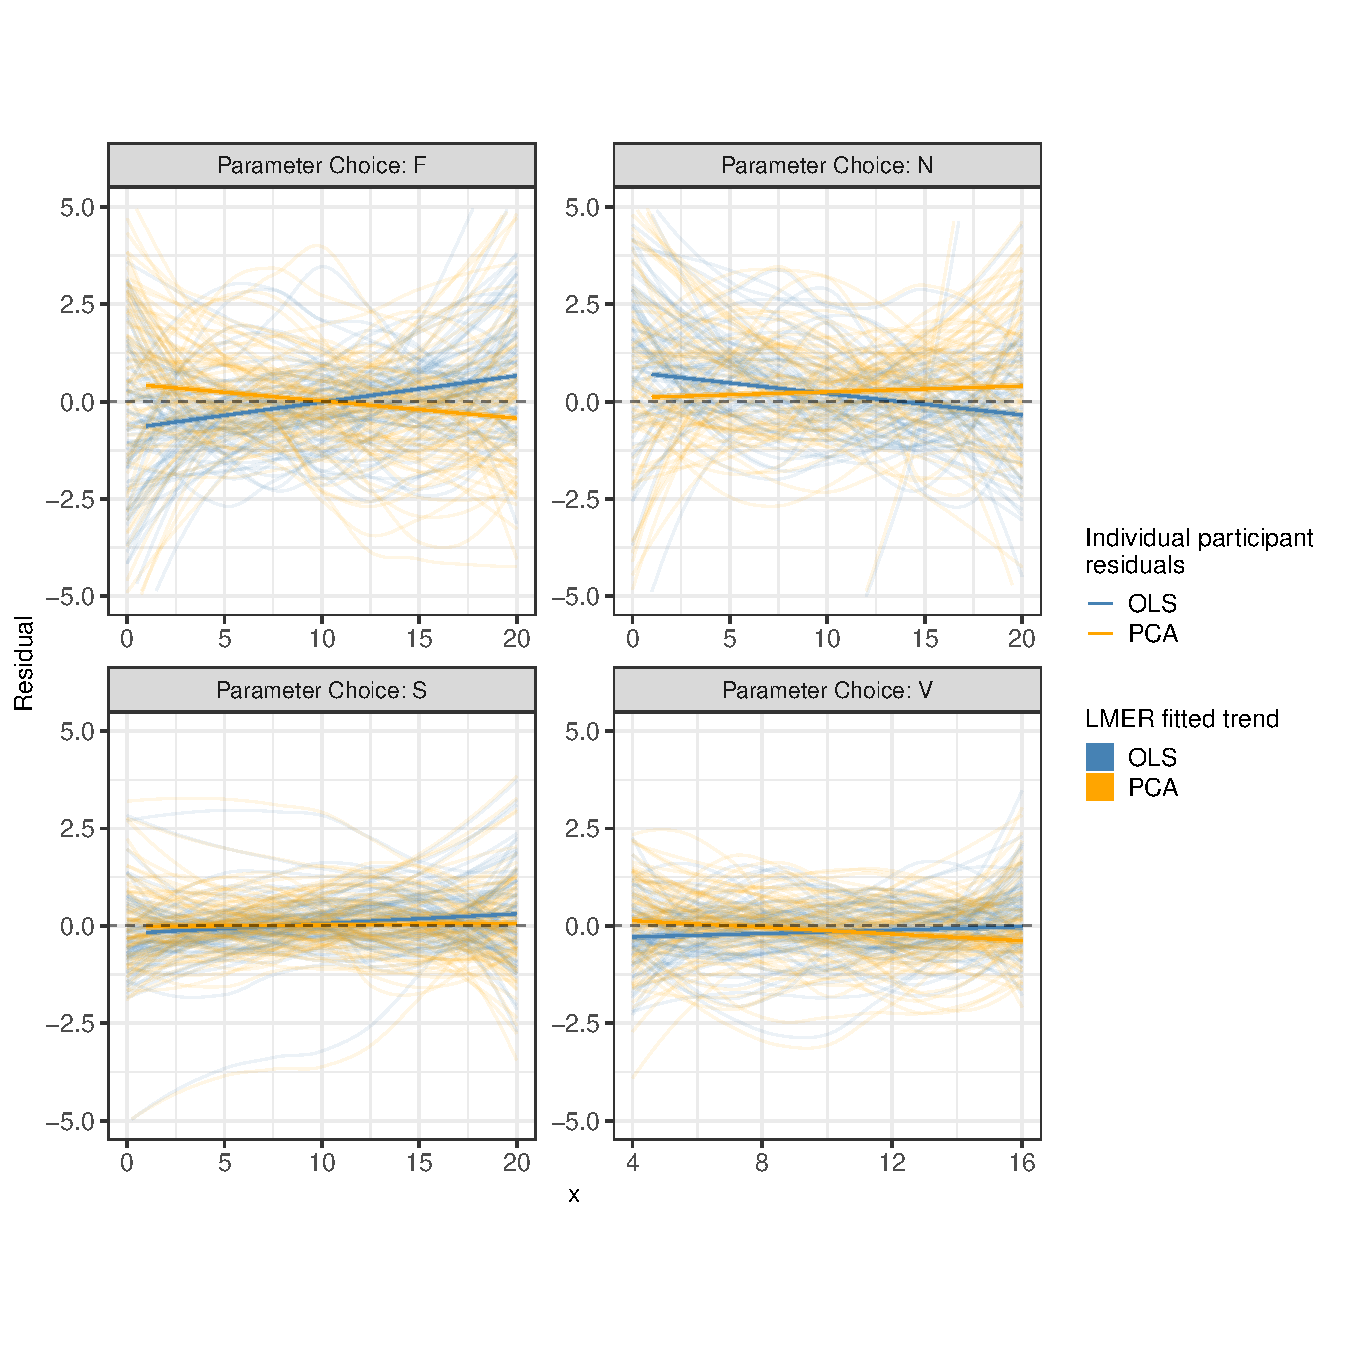
\includegraphics{./images/fig-eyefitting-lmer-residualplots-1.pdf}

}

\caption{\label{fig-eyefitting-lmer-residualplots}Estimated trends of
residuals (vertical deviation of participant drawn points from both the
OLS (blue) and PCA (orange) fitted points) as fit by the linear mixed
model. A random sample of 75 participants was selected to display the
individual participant residuals behind the overall trend.}

\end{figure}

Eliminating the linear trend constraint, we can extend the method and
analysis beyond ordinary least squares by using generalized additive
mixed models (GAMM) to estimate smoothing splines and allow for a more
flexible residual trend. The \texttt{bam} function in the \texttt{mgcv}
package was used to fit a GAMM separately to the OLS and PCA. Parameter
choice was treated as a fixed effect with no estimated intercept and a
separate smoothing spline for \(x\) was estimated for each parameter
choice. A random participant effect accounting for variation due to
participant and a random spline for each participant accounted for
variation in spline for each participant. The GAMM equation for each fit
(OLS and PCA) residuals is given by: \begin{equation}
y_{ijk, drawn} - \hat y_{ijk, fit} = e_{ijk,fit} = \alpha_i + s_{i}(x_{ijk}) + p_{j} + s_{j}(x_{ijk})
\end{equation} \noindent where

\begin{itemize}
\tightlist
\item
  \(y_{ijk,drawn}\) is the drawn y-value for the \(i^{th}\) parameter
  choice, \(j^{th}\) participant, and \(k^{th}\) increment of
  \(x\)-value
\item
  \(\hat y_{ijk,fit}\) is the fitted y-value for the \(i^{th}\)
  parameter choice, \(j^{th}\) participant, and \(k^{th}\) increment of
  \(x\)-value corresponding to either the OLS or PCA fit
\item
  \(e_{ijk,fit}\) is the residual between the drawn and fitted y-values
  for the \(i^{th}\) parameter choice, \(j^{th}\) participant, and
  \(k^{th}\) increment of \(x\)-value corresponding to either the OLS or
  PCA fit
\item
  \(\alpha_i\) is the intercept for the parameter choice \(i\)
\item
  \(s_{i}\) is the smoothing spline for the \(i^{th}\) parameter choice
\item
  \(x_{ijk}\) is the \(x\)-value for the \(i^{th}\) parameter choice,
  \(j^{th}\) participant, and \(k^{th}\) increment
\item
  \(p_{j} \sim N(0, \sigma^2_\text{participant})\) is the error due to
  participant variation
\item
  \(s_{j}\) is the random smoothing spline for each participant.
\end{itemize}

\begin{figure}

{\centering 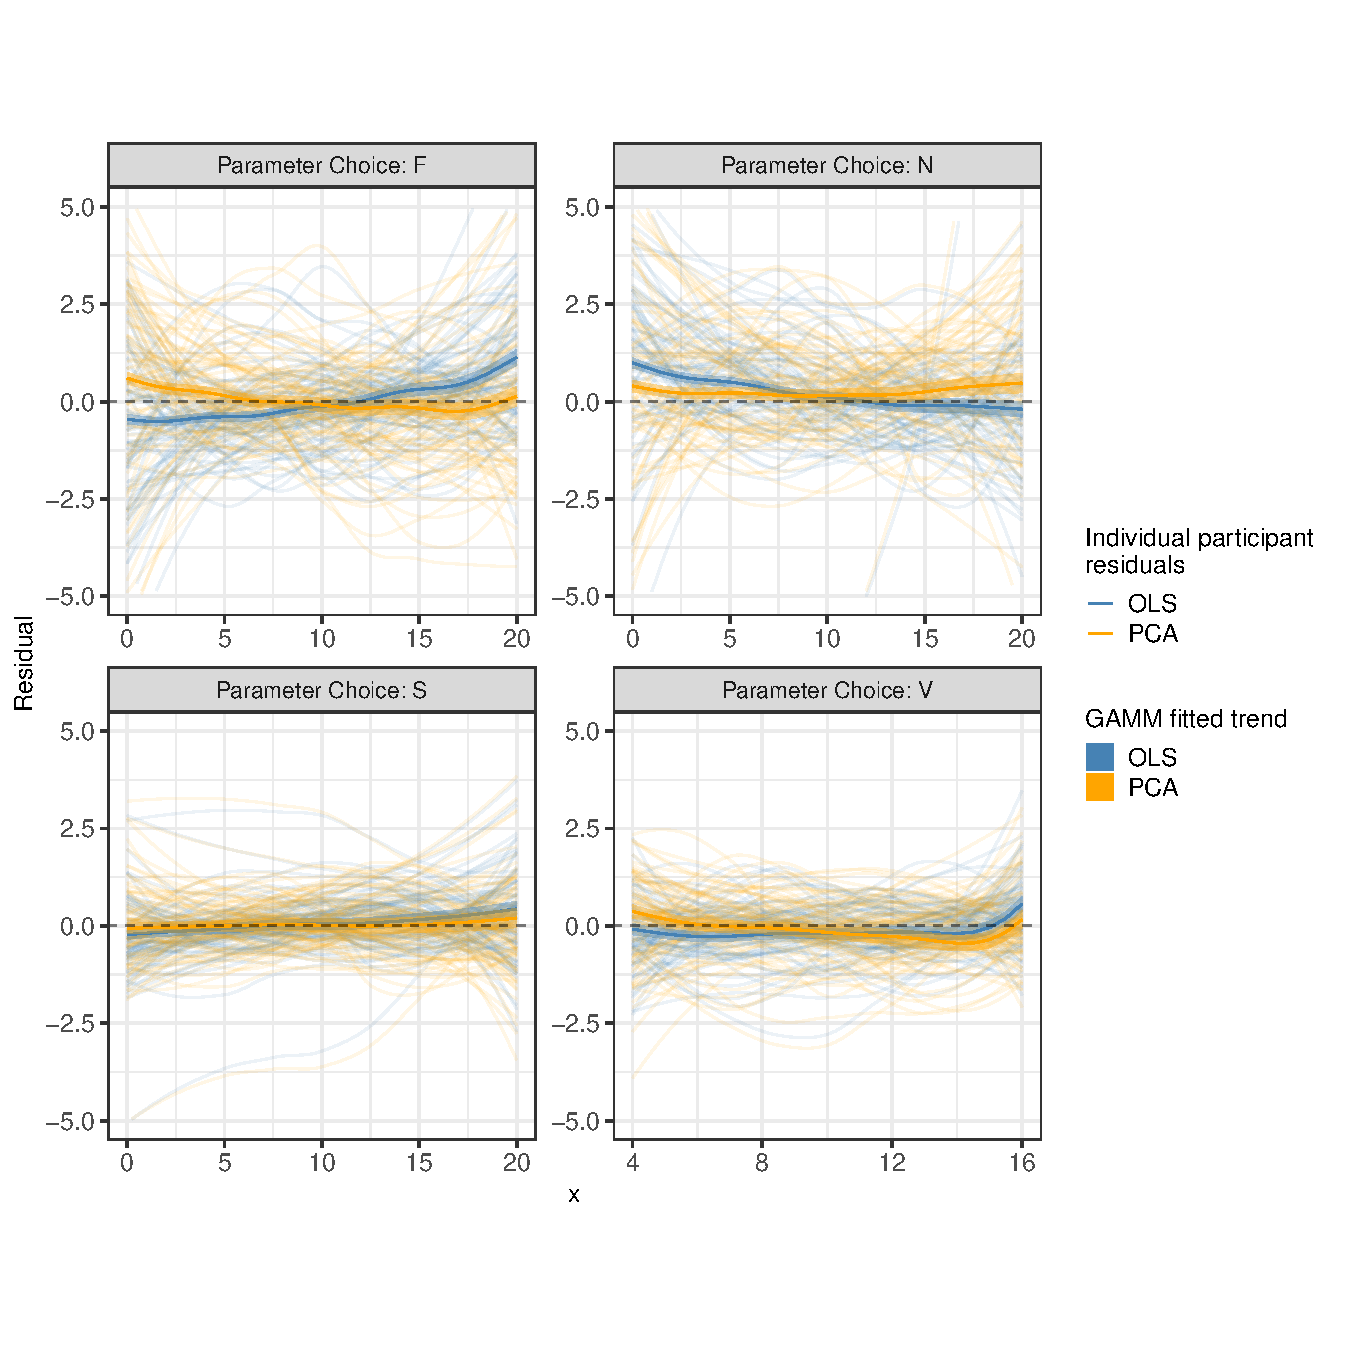
\includegraphics{./images/fig-eyefitting-gamm-residualplots-1.pdf}

}

\caption{\label{fig-eyefitting-gamm-residualplots}Estimated trends of
residuals (vertical deviation of participant drawn points from both the
OLS (blue) and PCA (orange) fitted points) as fit by the generalized
additive mixed model. A random sample of 75 participants was selected to
display the individual participant residuals behind the overall trend.}

\end{figure}

Figure~\ref{fig-eyefitting-lmer-residualplots} and
Figure~\ref{fig-eyefitting-gamm-residualplots} show a visual analysis of
the estimated trends of residuals (vertical deviation of participant
drawn points from both the OLS and PCA fitted points) as modeled by a
LMM and GAMM respectively. A random sample of 75 participants was
selected to display individual participant residuals behind the overall
residual trend. Examining the plots, the estimated trends of PCA
residuals (orange) appear to align more parallel and closer to the
\(y=0\) horizontal (dashed) line than the OLS residuals (blue). In
particular, this trend is more prominent in parameter choices with large
variances (F and N). Results from our study were consistent with those
found in the original study; when shown points following a linear trend,
participants tended to fit the slope of the first principal component
Our study established `You Draw It' as a method for graphical testing
and reinforced the differences between intuitive visual model fitting
and statistical model fitting, providing information about human
perception as it relates to the use of statistical graphics.

\hypertarget{extension-to-nonlinear-data}{%
\subsection{Extension to Nonlinear
Data}\label{extension-to-nonlinear-data}}

After validating the `You Draw It' method, we conducted a study
utilizing the new method to evaluate participants ability to make
forecasts for exponentially increasing data on log and linear scales.
Along with analyzing the feedback data with the GAMM method for
flexibility due to nonlinear data, we used spaghetti plots to conduct a
visual analysis of participant forecasts compared to the nonlinear least
squares statistical model and make comparisons between two chart design
features Figure~\ref{fig-exponential-yloess-spaghetti-plot-2-1}. This
study demonstrated the advantage of using the `You Draw It' method
paired with GAMM and visual analysis methods for measuring perception
and visual patterns of nonlinear data.

\begin{figure}

{\centering 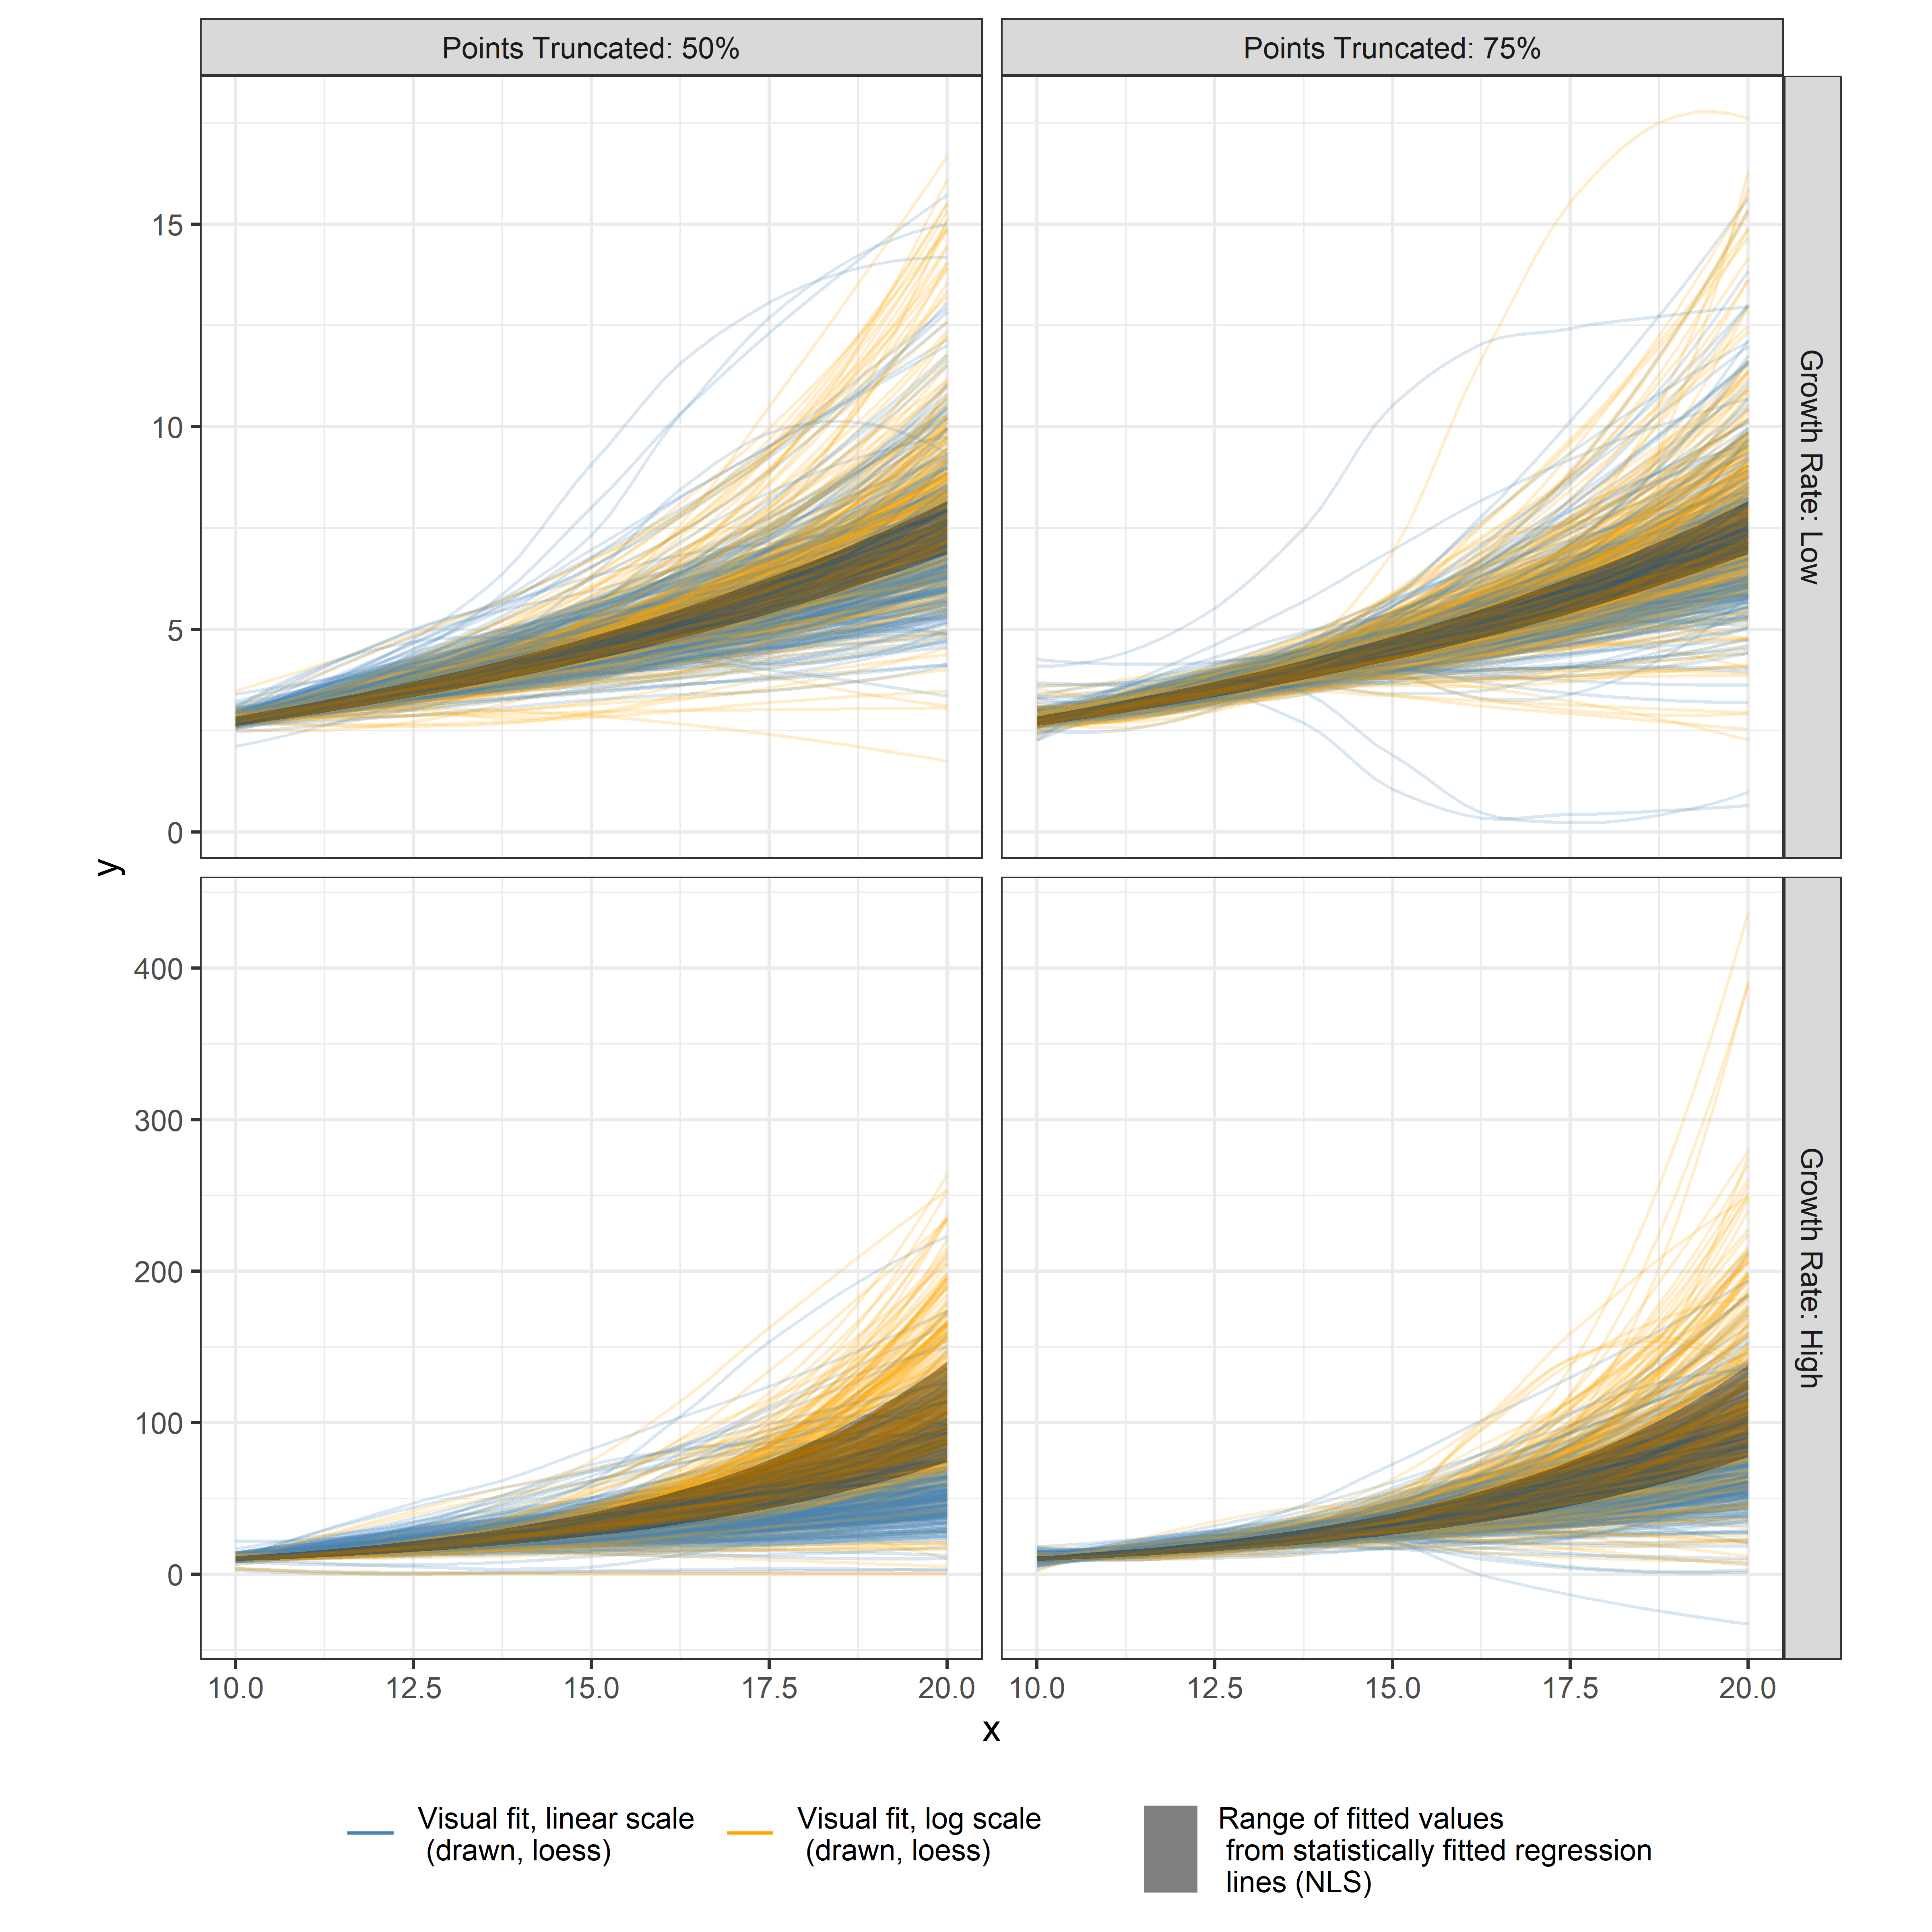
\includegraphics{images/exponential-yloess-spaghetti-plot-2-1.png}

}

\caption{\label{fig-exponential-yloess-spaghetti-plot-2-1}Spaghetti plot
of results from a study which asked participants to forcast trends of
exponentially increasing data. Participants drawn lines on the linear
scale are shown in blue and the log scale are shown in orange.
Variability in the statistically fitted regression lines occured due to
a unique data set being simulated for each individual; the gray band
shows the range fitted values from the statistically fitted regression
lines.}

\end{figure}

\hypertarget{conclusion}{%
\section{Conclusion}\label{conclusion}}

The data presented in this paper are part of a much broader experiment
on the perception of log scales; while this paper focuses primarily on
the computational implementation of the `You Draw It' method and its
adaptation to testing graphics, we are currently finishing the analysis
and description of the broader experiment, which uses this `You Draw It'
method to assess user prediction of exponential trends.

By introducing an interactive method for assessing eye-fit data
summaries, along with an analysis method which allows us to test
competing hypotheses to determine whether user responses are similar to
particular statistical models, we have provided another tool for
experimentally testing statistical charts. In the future, we hope to
create an R package to more easily facilitate these types of user
experiments, making this technique available to other researchers who
may not be willing to tinker with JavaScript directly.

As with any method for testing statistical graphics, there are a host of
additional studies which would be useful to understand how users react
to the `You Draw It' method and what parameters are most important for
the researcher to control. One avenue of future exploration is to
investigate the effect of axis limits on user anchoring. We know that
the perceptual experience is heavily affected by anchoring to e.g.~axis
breaks, and we would expect that a similar anchoring effect might be
present based on the limits of the plot and the amount of space in \(x\)
and \(y\) provided for the user to draw.

\svp{XXX add references to the anchoring bit XXX}

\hypertarget{references}{%
\section*{References}\label{references}}
\addcontentsline{toc}{section}{References}

\hypertarget{refs}{}
\begin{CSLReferences}{1}{0}
\leavevmode\vadjust pre{\hypertarget{ref-aisch2015you}{}}%
Aisch, Gregor, Amanda Cox, and Kevin Quealy. 2015. {``You Draw It: How
Family Income Predicts Children's College Chances.''} \emph{The New York
Times} 28.

\leavevmode\vadjust pre{\hypertarget{ref-lme4-pkg}{}}%
Bates, Douglas, Martin Mächler, Ben Bolker, and Steve Walker. 2015.
{``Fitting Linear Mixed-Effects Models Using {lme4}.''} \emph{Journal of
Statistical Software} 67 (1): 1--48.
\url{https://doi.org/10.18637/jss.v067.i01}.

\leavevmode\vadjust pre{\hypertarget{ref-bostock2011d3}{}}%
Bostock, Michael, Vadim Ogievetsky, and Jeffrey Heer. 2011. {``D\(^3\)
Data-Driven Documents.''} \emph{IEEE Transactions on Visualization and
Computer Graphics} 17 (12): 2301--9.

\leavevmode\vadjust pre{\hypertarget{ref-ciccione2021can}{}}%
Ciccione, Lorenzo, and Stanislas Dehaene. 2021. {``Can Humans Perform
Mental Regression on a Graph? Accuracy and Bias in the Perception of
Scatterplots.''} \emph{Cognitive Psychology} 128: 101406.

\leavevmode\vadjust pre{\hypertarget{ref-finney1951subjective}{}}%
Finney, DJ. 1951. {``Subjective Judgment in Statistical Analysis: An
Experimental Study.''} \emph{Journal of the Royal Statistical Society:
Series B (Methodological)} 13 (2): 284--97.

\leavevmode\vadjust pre{\hypertarget{ref-mosteller1981eye}{}}%
Mosteller, Frederick, Andrew F Siegel, Edward Trapido, and Cleo Youtz.
1981. {``Eye Fitting Straight Lines.''} \emph{The American Statistician}
35 (3): 150--52.

\leavevmode\vadjust pre{\hypertarget{ref-r-software}{}}%
R Core Team. 2022. \emph{R: A Language and Environment for Statistical
Computing}. Vienna, Austria: R Foundation for Statistical Computing.
\url{https://www.R-project.org/}.

\leavevmode\vadjust pre{\hypertarget{ref-usenergyinformationadministrationWeeklyAllGrades2022}{}}%
US Energy Information Administration. 2022. {``Weekly {U}.{S}. {All}
{Grades} {All} {Formulations} {Retail} {Gasoline} {Prices} ({Dollars}
Per {Gallon}).''} \emph{US Energy Information Administration Independent
Statistics \& Analysis}.
\url{https://www.eia.gov/dnav/pet/hist/LeafHandler.ashx?n=PET\&s=EMM_EPM0_PTE_NUS_DPG\&f=W}.

\end{CSLReferences}



\end{document}
